
%\documentclass[a4paper, 11pt, twocolumn, notitlepage]{article}
\documentclass[a4paper, 11pt, notitlepage]{article}

\usepackage{amsmath}
\usepackage{amsthm}
\usepackage{amssymb}

\usepackage{cite}
\usepackage{cleveref}

\usepackage{url}

\usepackage{graphicx}

\usepackage{pdfpages}

\title{Computational Intelligence Lab:\\Sentiment Analysis Project}
\author{Teymur Babayev babayevt@student.ethz.ch \and Misels Kaporins miselsk@student.ethz.ch \and Pius von D\"aniken piusv@student.ethz.ch \\
Team: greentshirt \\
Department of Computer Science, ETH Z\"urich, Switzerland
}
\date{Spring 2016}


\begin{document}

\maketitle

\begin{abstract}
    \textit{GloVe} and similar word embeddings are useful to measure semantic
    similarities on the word level. We try to create sentence level features
    based on a clustering of word vectors and test whether they can help
    improve the accuracy on a text classification task. We find that this is not
    the case.
\end{abstract}


\section{Introduction}

\subsection{Sentiment Analysis}

In sentiment analysis we want to extract subjective information from text. It is
usually formulated as a text classification task where we want to distinguish
text sections by the attitude of the speaker or author. A sentence like
\textit{Just got my midterm and I'm impressed!} might be categorized as `positive'
whereas \textit{Exams are coming soon.} might be considered `negative'.

For our application we try to classify tweets into `positive' and `negative'
categories based on whether the contain a happy (`:)') or sad (`:(') smiley.

Real time sentiment analysis of social media posts in general can be particularly
useful for public relations and marketing purposes as it can provide insight into
customer satisfaction and related metrics.

\subsection{Baselines}

Most modern state of the art text classification systems are based on convolutional
neural networks. We will use a simple convolutional neural network similar to
the one presented in~\cite{cnn14} as a baseline for comparison.

As a second baseline we use a traditional feature based classifier. We extract
tfidf (term frequency-inverse document frequency) features from the tweets
and train a tree ensemble classifier using gradient boosting~\cite{gradBoost}.

\subsection{Contribution}

For our main contribution we extract additional features based on a clustering
of the vector space embedding of the words in a tweet. We first compute global
vectors~\cite{glove} for the words in our dataset and use simple k-means to cluster them.  



\section{Models and Implementation}

\subsection{Convolutional Neural Network}

\begin{figure}
    \centering
    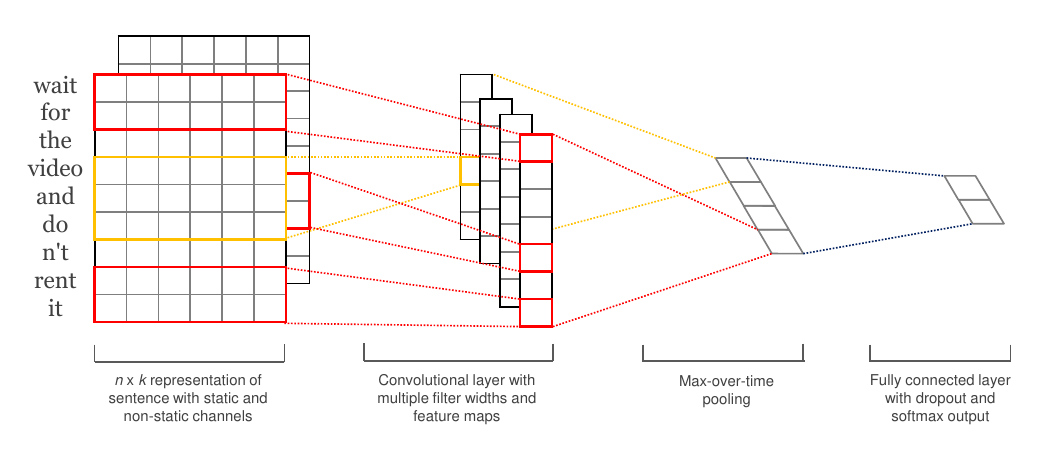
\includegraphics[height=1.9in]{text_cnn.png}
    \caption{CNN Architecture For Text Classification~\cite{cnn14}}\label{fig:arch}
\end{figure}

The basic structure of the CNN we use can be seen in~\cref{fig:arch} which is
taken directly from~\cite{cnn14}. Every tweet will be split in a sequence of $n$
words $\left(w_1, w_2, \dots, w_n\right)$. For shorter tweets we pad the sequence
with a special pad word $w_{pad}$. Every word $w_i$ is associated with an embedding
vector $\mathbf{x}_{w_i} \in \mathbb{R}^k$.

These embedding vectors can either be static
and come from a pretrained embedding, such as \textit{word2vec}~\cite{word2vec}
or \textit{GloVe}~\cite{glove}, or be dynamically adapted during training.

Each tweet has therefore a representation $\mathbf{X} \in \mathbb{R}^{n \times k}$. Let
$\mathbf{W} \in \mathbb{R}^{h \times k} h \le n$ and
$v_t = \sum_{i = t}^{t + h}\sum_{j = 0}^{k} \mathbf{W}_{i,j} \mathbf{X}_{i,j}$ $\forall 1 \le t \le n - h + 1$.
The resulting vector $\mathbf{v}$ is the convolution of $\mathbf{X}$ and $\mathbf{W}$.
Furthermore let $c_t = f\left(v_t + b\right)$ where $f$ is some non-linear function
and $b \in \mathbb{R}$ a bias term. The resulting vector $\mathbf{c} \in \mathbb{R}^{n - h + 1}$ is called
a feature map.

The feature map $\mathbf{c}$ is then maxpooled which means we select $\hat{c} = \max_{t}\left\{c_t\right\}$.

This process shows how we extract one feature $\hat{c}$ using one filter $\mathbf{W}$.
We use several filters with possibly different heights $h$ in parallel to get
a feature vector $\mathbf{\hat{c}}$, which is then fed into a fully connected
neural network to predict the correct label~\cite{cnn14}~\cite{cnnBlog}.

We based our implementation of the described network on~\cite{cnnBlog} and~\cite{cnnImpl}.
We chose filter lengths $3$, $4$, $5$ and $6$. For each filter length we used
$128$ different filters, resulting in a total of $512$ features.
We initialize the filter parameters and embedding vectors with gaussian
random vectors. We use a dropout rate of $0.5$ for regularization.

\subsection{TF-IDF}

This model is based on the bag of words assumption where each document is
represented by the multiset of words it contains. \textit{TF} stands for
\textit{term freqruency} and measures how often a certain word $w$ appears in
a specific document $d$. Given some document $d$ of length $n$, $d = {\left\{w_i\right\}}_{i = 1}^{n}$
we have $tf\left(w, d\right) = \frac{|\left\{w_i = w | 1 \le i \le n\right\}|}{n}$

\textit{IDF} stands for the \textit{inverse document frequency}
where the \textit{document frequency} measures in how many documents $w$ appears
at least once given some corpus of documents
$\mathcal{C}$. $idf\left(w, \mathcal{C}\right) = \frac{|\mathcal{C}|}{|\left\{d \in \mathcal{C} | w \in d\right\}|}$.
%In order to avoid a division by $0$ on previously unseen terms we add a dummy
%document containing every word and get: $idf\left(w, \mathcal{C}\right) = \frac{|\mathcal{C}| + 1}{|\left\{d \in \mathcal{C} | w \in d\right\}| + 1}$

In its simplest form the \textit{TF-IDF} score of a word $w$ given a document $d$
and corpus $\mathcal{C}$ is $tfidf\left(w, d, \mathcal{C}\right) = tf\left(w, d\right)idf\left(w, \mathcal{C}\right)$.

Using this we can build a sparse feature vector $\mathbf{x}_d \in \mathbb{R}^{|\mathcal{V}|}$
for some document $d$ where $\mathcal{V}$ is the set of all words in the whole
corpus $\mathcal{C}$.

We use these features to train a tree ensemble using gradient boosting~\cite{gradBoost}.

\subsection{GloVe Cluster Features}

Methods such as \textit{GloVe}~\cite{glove} and \textit{word2vec}~\cite{word2vec}
embed words in an euclidean vector space, suggesting that similar words are 
closer together in that space.

Assume we have an embedded vector $x_w \in \mathbb{R}^{m}$ for each word $w$ in our vocabulary.
We cluster these vectors using \textit{k-means} and get a clustering
$c : \mathbb{R}^{m} \rightarrow \left\{1, 2, 3, \dots, k\right\}$.
Given a document $d$ of length $n$, $d = {\left\{w_i\right\}}_{i = 1}^{n}$,
we can construct the following features: $f_j = \frac{|\left\{w \in d | c\left(x_w\right) = j\right\}|}{n}$
for $1 \le j \le k$.

The features $f_j$ represent the normalized histogram of words in the document belonging to
a certain cluster $j$ of words.

When training \textit{GloVe} vectors we used an embedding dimension of $128$ and
trained the model for $10$ epochs.




\section{Experiments}

\subsection{Dataset}

The dataset consists of a total of $2.5$ million tweets of which half belong to
the positive and half to the negative class. The validation set consists of
$10000$ unlabeled tweets.

We used the whole training data set to build the
vocabulary, compute \textit{GloVe}~\cite{glove} vectors and train the 
convolutional neural network but only used $100000$ samples of each class to
train the ensemble classifiers.

\subsection{Preprocessing}

To prepare the data we first compute a mapping from words to integer ids. This
allows us to operate on sequences of integers instead of sequences of strings.
In order to reduce the size of the vocabulary we remove stopwords using a list
of stopwords. Furthermore we stem all words and filter words that only appear
rarely.

\subsection{Results}

\begin{table}[h]
    \centering
    \begin{tabular}{l r}
        Method & Classification Accuracy in \% \\
        \hline
        CNN & $76.76$\% \\
        tfidf & $81.5$\% \\
        GloVe cluster histograms & $61.74$\% \\
        tfidf \& clusters & $81.86$\% \\
        tfidf \& clusters\footnotemark{} & $82.22$\% \\
    \end{tabular}
    \caption{Different Models Evaluated On The Kaggle Public Leaderboard}\label{tab:res}
\end{table}
\footnotetext{using the same features but $3000$ instead of $1000$ trees in the ensemble} 

\Cref{tab:res} shows the classification accuracy of the different models on the
validation set as reported by the public leaderboard of the Kaggle competition.

We can clearly see that the GloVe cluster histograms bring no significant
improvement over the simple tfidf features. Moreover they perform significantly
worse when used on their own.

Surprisingly the convolutional neural network performs worse than the tfidf model
as well.

A possible reason for the cluster histogram features to perform this badly is that
a lot of important antonyms fall into the same cluster. For example the words
`happy', `sad', `good', `bad', `excited' tend to consistently fall into the
same cluster. Increasing the number of clusters does not help since even when
we increase the number of clusters to $1000$ usually less than $100$ contain
more than a single word.


\bibliography{refs}
\bibliographystyle{plain}

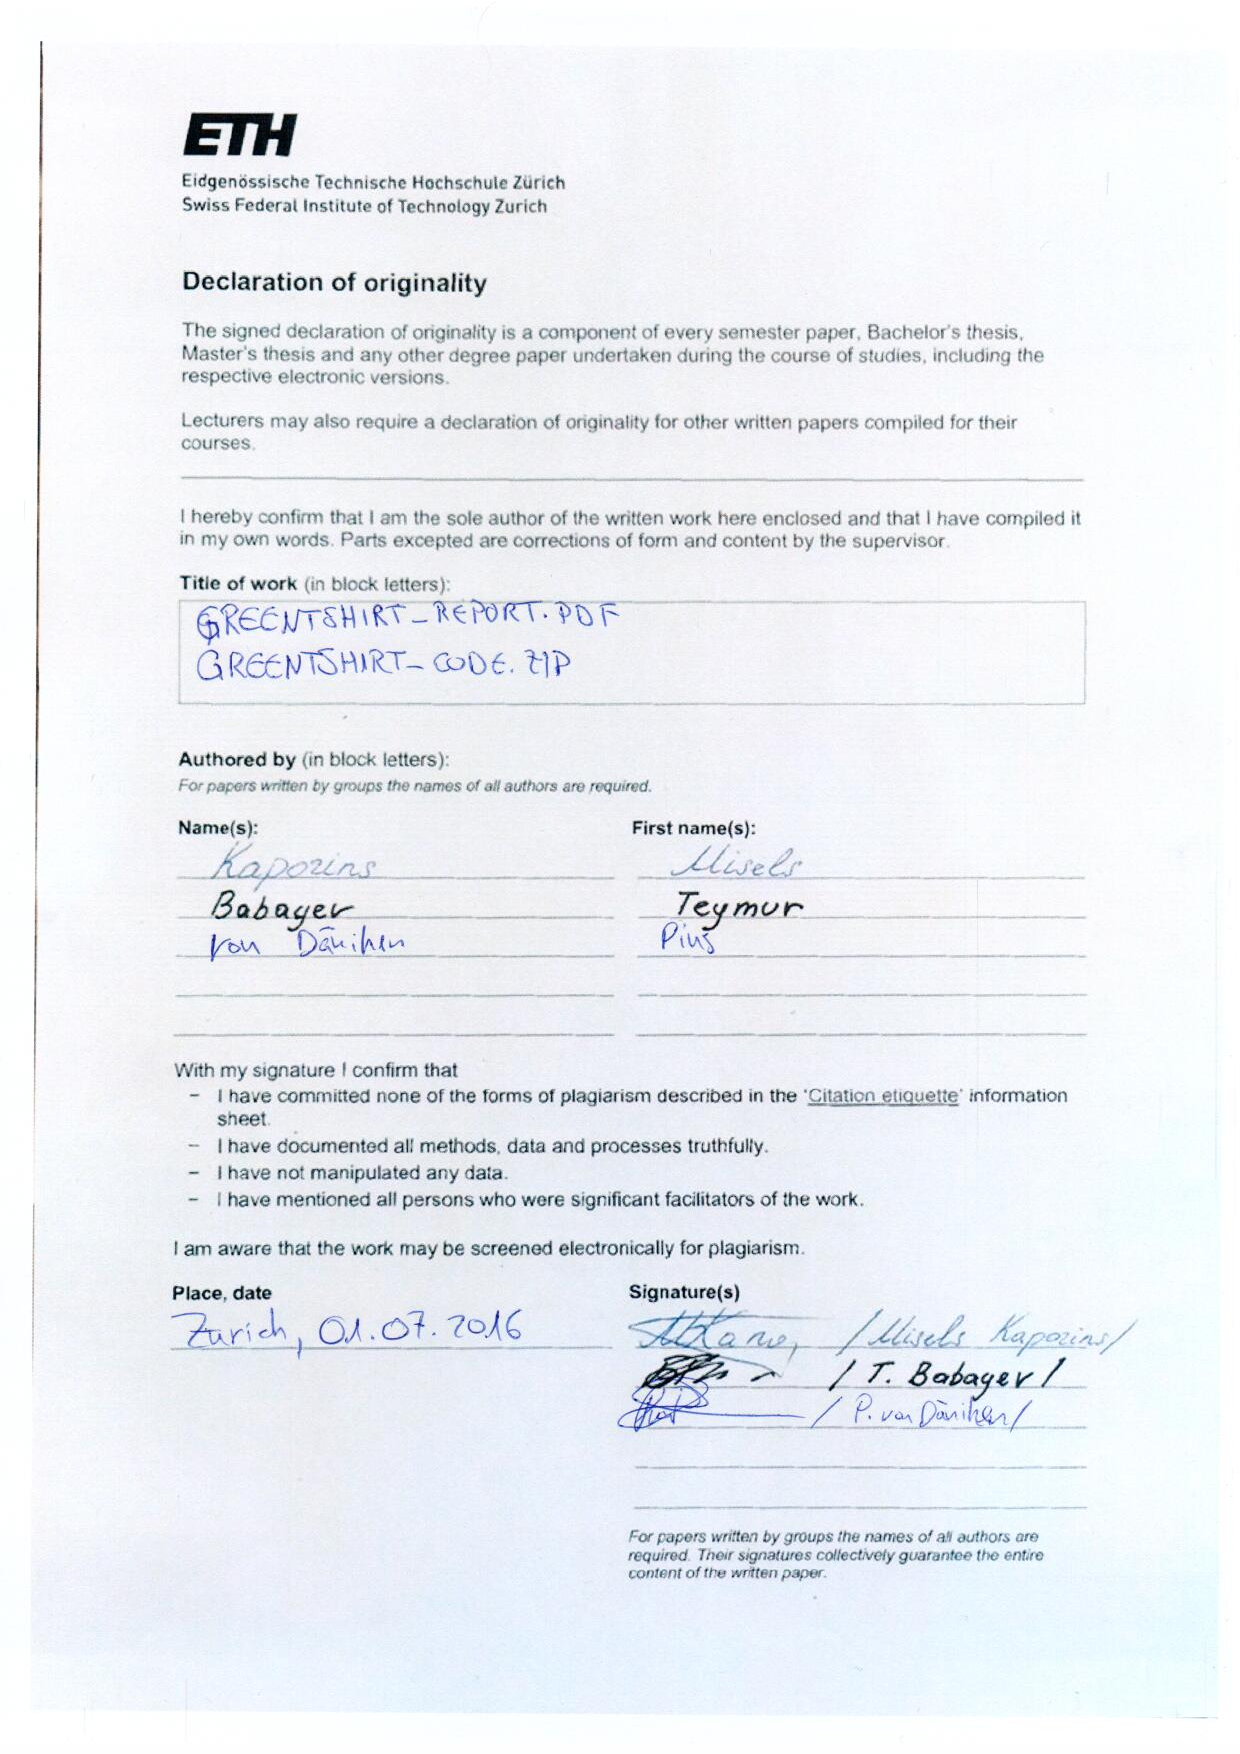
\includepdf{declaration_of_originality.pdf}

\end{document}
